\chapter{Disseny del \est{firmware}}

En aquest capítol es detallarà tot el que té a veure amb el codi que anirà dintre 
de la placa de circuit imprès realitzada en el capítol anterior. Com que les
connexions entre la placa creada i l'entorn de proves amb la placa \est{Digispark}
i el mòdul \est{GY521} són idèntiques, el \est{firmware} o microprogramari que 
es creï servirà per a les dues plaques.

\section{Proves prèvies del projecte \est{i2c\_tiny\_usb}}
\label{sec:testinc-i2c-tiny}

Tal com s'ha dit en l'apartat \ref{subsec:hw_digispark}, es va descobrir
el projecte \est{i2c\_on\_usb} \cite{I2cTinyUsb}.
Aquest projecte ha aconseguit dissenyar
una placa molt semblant a la de \est{Digispark} i, mitjançant programari (tant
del cantó del microcontrolador com afegint controladors al \est{kernel} de
Linux), el dispositiu s'identifica com un mestre \acro{i2c} de cara a
l'ordinador, i apareix a \fitx{/dev/i2c-X}, en què X és el número de dispositiu.

A \cite{i2cOnLittleWireBuilding} s'ha trobat el projecte
\est{i2c\_on\_littlewire}, una adaptació de
\est{i2c\_tiny\_usb} per a la placa \est{Digispark}, acompanyat d'un tutorial 
molt detallat sobre com programar la placa.
Aquest projecte ha anat molt bé per fer proves de precisió del sensor a més
alt nivell (per exemple, utilitzant la llibreria \acro{i2c} de Python). Tanmateix,
es va descartar utilitzar-lo per a aquest treball per dos motius:

\begin{itemize}
    \item Aquest \acro{tfg} pretén ser el més versàtil possible i utilitzar
    els estàndards de més alt nivell. En el capítol anterior s'ha comentat que
    es volien utilitzar les classes \acro{hid} i el mòdul \acro{iio}. El projecte
    \est{i2c\_tiny\_usb} utilitza programari propi i, tot i que estigui inclòs
    en el \est{kernel} de Linux \cite{I2cTinyKernel}, s'hauria de fer de zero
    per a altres sistemes operatius.
    \item L'objectiu del \acro{tfg} és aprendre durant el procés de
    desenvolupament. Si s'agafa un projecte que ja ho té tot fet no s'adquirirà
    experiència en aquests camps.
\end{itemize}

Tot i haver descartat el projecte \est{i2c\_on\_littlewire}, es va considerar
oportú demostrar que una lectura del sensor amb aquest dispositiu era viable.
Es va partir dels exemples disponibles a \cite{I2cTinyUsb}, que consisteixen en
un codi en C que utilitza \est{libusb} per llegir dades del sensor. Només va
fer falta adaptar la implementació del sensor (basant-se en els seus requisits,
explicats en detall a l'apartat \ref{subsec:i2c_sensor}).

Es van poder llegir les mesures del sensor sense gaires complicacions, però també
es va modificar el programa per deixar d'utilitzar \est{libusb} i es va fer servir,
en canvi, \est{libi2c}, la llibreria de Linux per comunicar-se amb dispositius
\acro{i2c}. Aquesta també es pot utilitzar des de llenguatges de més alt nivell,
com Python.

\section{Creació d'un entorn de desenvolupament}

Per poder desenvolupar amb comoditat el \est{firmware} del projecte, és crucial
facilitar la tasca de provar les modificacions fetes. Per aquest motiu, s'ha
planejat tot un entorn de treball que es detalla en aquest apartat.

\subsection{Programació del microcontrolador}
\label{subsec:bootloader}

Hi ha diverses formes de programar el microcontrolador, però la més adequada
per al sistema en qüestió, i tenint present que es voldrà programar el dispositiu
diverses vegades, és utilitzar un \est{bootloader} que identifiqui el dispositiu
com una placa programable durant els primers segons d'operació. Si poc després 
que el dispositiu no estigui alimentat l'usuari no ha intentat programar-hi res 
a través de l'ordinador, s'executarà el programa principal del microcontrolador.

Aquest \est{bootloader} que s'ha descrit és exactament el que hi ha en la
placa \est{Digispark} per defecte. Com és evident, en un producte definitiu no
interessa posar un \est{bootloader} que retardi el començament del programa
uns segons més, però per fer proves valdrà la pena aquesta espera.

Programar el \est{Digispark} o una placa equivalent com la d'aquest projecte
utilitzant el \est{bootloader} definit anteriorment és una tasca molt senzilla.
Un cop es disposi del fitxer \fitx{.hex} que es vol programar al
microcontrolador, es poden utilitzar programes com \ord|avrdude| o
\est|micronucleus| perquè, mentre s'estigui executant el \est{bootloader}, es 
reprogrami el xip \cite{DigisparkBootloader}.

Per programar la placa amb un sistema basat en Linux s'ha de dur a terme una
tasca extra: els permisos. Un usuari administrador podrà programar la placa
sense cap problema, però executar com a \est{root} un programa sempre implica
assumir riscos. Per això, el més recomanat és crear una regla \acro{udev}
per al dispositiu en qüestió, fent que sigui accessible per a tots els usuaris.
Es pot consultar un tutorial detallat a \cite{CreateUdevRules}.

\subsection{Automatització del procés de compilació i programació}

Un cop se sap com programar la placa, el següent pas a seguir és crear un
\est{Makefile} per poder compilar i programar amb una única comanda.
No és la primera ni la segona vegada que s'utilitza l'eina \ord|make| en
aquesta titulació, però sí que és la primera vegada que s'utilitza amb una placa
que no sigui un Arduino. Tanmateix, no hi ha gaire diferència, tret de la
part de programar mencionada en l'apartat anterior.

S'ha preparat i documentat el \est{Makefile} com es mereix: s'ha posat un menú
d'ajuda, s'ha posat l'opció per programar els fusibles del microcontrolador
(aquesta part només s'ha de fer una vegada), s'han posat opcions per
eliminar tots els fitxers generats i també per poder depurar el programa.

\section{Comunicació amb l'ordinador mitjançant USB}

Amb l'entorn de programació preparat, ja es pot començar a crear el
\est{firmware} del projecte. Es començarà per la part més complicada: la
llibreria \acro{v-usb}. Tanmateix, està molt ben documentada i disposa de
tutorials disponibles a internet.

La tasca d'aquest apartat és aconseguir que l'ordinador identifiqui la placa
com un acceleròmetre tridimensional. Per arribar a aquesta meta hi haurà un
seguit de reptes i barreres a superar.

El punt de partida és els codis d'exemple del repositori del projecte
\cite{VusbProjects}.
També hi ha un repositori amb bastants exemples, però la majoria només són
compatibles amb un \acro{AtMega}, i s'haurien d'adaptar de totes maneres.

\subsection{Calibratge de l'osci\l.lador del microcontrolador}

Un dels problemes més grans del microcontrolador que s'està utilitzant és que
l'osci\l.lador intern que disposa no és compatible amb el que demana el
protocol \acro{usb}. Es disposa d'una freqüència de
\SI[round-mode=places,round-precision=1]{16.5}{\mega\hertz} i
\acro{usb2} funciona a
\SI[round-mode=places,round-precision=0]{1}{\kilo\hertz}.

Aquest problema és ben conegut pels desenvolupadors de \acro{v-usb} i, en alguns
dels exemples, s'explica com s'ha de calibrar l'osci\l.lador intern per poder-se
comunicar amb \acro{usb2} basant-se en els intervals de temps entre els que es
rep senyal des de l'ordinador. Es recomana consultar aquests codis
\cite{Vusb} si es vol entendre millor aquest apartat.

No utilitzar un rellotge compatible amb el protocol \acro{usb} viola les normes
marcades per la mateixa entitat \acro{usb-if}. Tanmateix, com s'ha vist en
apartats anteriors, no es pretén certificar com a \acro{usb} el dispositiu
(per altres motius no tècnics), per la qual cosa, mentre funcioni correctament 
en l'àmplia majoria de dispositius, es considerarà un èxit.

\subsection{Identificadors USB durant el desenvolupament}

En aquest punt del projecte és quan s'ha de decidir
quin \acro{vid-pid} es posa al dispositiu, si més no, durant el temps de
desenvolupament. Tal com s'ha vist en l'apartat \ref{subsec:usb-if}, hi ha dues
opcions possibles.

Durant el desenvolupament es decidirà utilitzar un parell de codis sense
consensuar-ho amb ningú. Aquesta és la solució més senzilla i ràpida, ja que per
obtenir identificadors a partir d'entitats mencionades anteriorment se sol
tardar un temps i acostumen a acceptar únicament projectes acabats o en fase
de proves finals.

Així doncs, s'ha optat per agafar el \acro{vid-pid}
\texttt{0x16c0}-\texttt{0x09e8}, que és la
parella de codis que els autors de \acro{v-usb} ofereixen per fer proves
individuals \cite{Vusb}. En altres paraules, \est{ObDev}, el propietari dels
codis, no assignarà mai aquests identificadors a un producte que acabi sent
comercialitzat. Va perfecte, doncs, per fer proves durant el desenvolupament del
projecte.

\subsection{Robustesa del \est{firmware}: \est{Watchdog}}

Una altra de les funcionalitats afegides en aquest projecte és el \est{watchdog}.
Es tracta d'un perifèric disponible en la majoria dels xips de l'arquitectura
\acro{avr} (entre d'altres) que té per objectiu detectar anomalies durant
l'execució del programa.

Un \est{watchdog} disposa d'un temporitzador que el programa principal ha d'anar
reiniciant cada poc temps. Si passa més d'un llindar de temps sense que el
temporitzador hagi sigut reiniciat, es considera que el programa principal s'ha
quedat penjat i el \est{watchdog} actua. Es pot configurar perquè actuï de
diferents maneres, però la més senzilla i popular és reiniciant el programa
sencer amb un \est{flag} activat, perquè el mateix programa pugui detectar que
no ha sigut un reinici voluntari, sinó a causa d'un error previ \cite{Watchdog}.

La llibreria \acro{v-usb} disposa d'exemples on s'utilitza un \est{watchdog} i,
per tant, no ha sigut gaire complicat afegir-lo en aquest projecte. És una
protecció addicional per assegurar-se que el dispositiu sempre funciona
correctament o, com a mínim, sense errors greus que no permetin l'execució
normal del programa.

\subsection{Implementació del sensor HID}

Finalment, la tasca més complicada d'implantar aquesta llibreria en el marc
del treball de final de grau és la configuració del nou tipus \acro{hid}:
acceleròmetre tridimensional.

Els tutorials trobats documenten molt bé com configurar tota la llibreria,
però no és feina seva explicar com es creen o modifiquen els \est{Hid Report Descriptors}.
Tot i que hi ha exemples amb la llibreria que utilitzen la classe \acro{hid},
aquests són per simular teclats o ratolins. S'ha hagut de fer molta recerca per
trobar una mica d'informació al respecte.

Tanmateix, després de molta prova i error i d'anar depurant amb l'ajuda de
\est{wireshark} totes les comunicacions (es recomana configurar \est{wireshark}
seguint aquest tutorial per rebre paquets \acro{usb}
\cite{InstallWireshark}), s'ha aconseguit
generar un \est{Hid Report Descriptor} que l'ordinador llegeix correctament.
Una de les referències més importants sobre aquesta part és \cite{VusbProjects}.

\section{Comunicació amb el sensor}

Un cop solucionada la comunicació entre el microcontrolador i l'ordinador, toca
centrar-se en la comunicació entre el microcontrolador i el sensor que, tal
com s'ha dit en el capítol anterior, es farà mitjançant el protocol \acro{i2c}.
En aquest apartat es defineix aquest protocol en el context de l'arquitectura
\acro{avr} i es detallen les peculiaritats i afegits que el sensor que
s'utilitza per al projecte requereix.

\subsection{Protocol I2C en l'arquitectura AVR}

El protocol \acro{i2c} utilitza dues línies bidireccionals, una per a les dades 
i una per al rellotge, que es connecten a 
\SI[round-mode=places,round-precision=0]{0}{\volt} o es deixen a l'aire (i els 
\est{pull-ups} la porten a la tensió d'alimentació).

Si bé hi ha moltes llibreries per a la placa Arduino i altres microcontroladors
de l'arquitectura \acro{avr}, totes utilitzen perifèrics específics que, en el
cas de l'\acro{AtTiny85} d'aquest projecte, o ja estan en ús per \acro{v-usb}, o
no existeixen per a aquest xip. Així doncs, s'ha d'aprendre el funcionament a
baix nivell del protocol i implementar-lo des de zero.

Per sort, aquest protocol no és gaire extens i amb unes 300 línies de codi en C
s'ha pogut implementar el parell de funcions que es necessitava per dur a
terme el projecte.

El protocol \acro{i2c}, tal com s'ha dit anteriorment, és molt versàtil i permet 
tolerar dispositius amb diferents tensions d'alimentació, més dispositius
(esclaus, però també mestres) i molta escalabilitat. El mestre és qui inicia
la transmissió (per tant, dos esclaus no poden parlar entre si), però la
direcció del flux de dades pot canviar \cite{I2c}.

El funcionament d'\acro{i2c} es pot resumir en poques paraules: el mestre envia
pel canal una adreça de 7 bits per saber amb quin dispositiu vol comunicar-se.
Aquests 7 bits són l'adreça del dispositiu, disponible als \est{datasheets}. Per
al sensor d'aquest projecte, l'adreça és \texttt{0x68} \cite{MPU6050reg}.
Després d'aquests 7 bits,
s'envia un vuitè bit, que dependrà de si es vol enviar dades o rebre dades del
dispositiu.

Un cop rebut el \est{acknowledgement} de l'esclau, comença la transmissió de
dades, que acabarà en funció dels valors de \est{acknowledgement} del mestre, o
de si el mestre envia un senyal de stop. Es recomana llegir el \est{dataheet} del
sensor a \cite{mpu6050specs} per entendre el funcionament de \acro{i2c},
ja que està molt ben explicat.

\subsection{Peculiaritats del sensor \est{MPU6050}}
\label{subsec:i2c_sensor}

Pel cas concret del sensor d'aquest projecte, hi ha un parell de normes extres
a part de les que estableix el protocol \acro{i2c} que serveixen per comunicar-se
d'una forma fiable amb el sensor.

El sensor \est{MPU6050} defineix en el seu \est{datasheet} un seguit de
registres que funcionen de la mateixa forma que els perifèrics en \acro{avr}:
no són registres comuns per guardar dades, sinó que és com si hi hagués una
extensió en els perifèrics del propi microcontrolador. Així doncs, si es llegeix
els registres \texttt{0x42:0x41}, es podrà consultar el valor mesurat de temperatura
(sense processar) \cite{MPU6050reg}. També es pot escriure en alguns registres,
per exemple, per activar o calibrar el sensor.

Per escriure en un registre només cal enviar per \acro{i2c} (és a dir, escriure)
l'adreça del registre i el valor a escriure. Si s'envien més bytes, el sensor
entendrà que s'han d'escriure en els registres posteriors. Pel que fa a la lectura,
s'ha de trametre l'adreça del registre i tornar a escriure la capçalera \acro{i2c},
però en aquest cas, en mode de lectura. El sensor enviarà els continguts del
registre en qüestió. Si es decideix de seguir llegint (mitjançant un \acro{nack}),
el sensor enviarà el valor del registre posterior \cite{mpu6050specs}.

Finalment, cal destacar que, pel que fa al sensor, poca configuració se li ha de
fer per rebre dades d'acceleració. Només cal desactivar el mode \est{sleep},
que ve sempre activat per defecte per estalviar energia, i començar a llegir
dades. Per als propòsits d'aquest projecte no és rellevant la freqüència de
dades, qualsevol serà suficient. La precisió de les dades tampoc és tan rellevant
per als càlculs que s'hauran de realitzar.

Per desenvolupar aquesta part del programa s'ha agafat com a referència el
codi de la llibreria d'Arduino per comunicar-se amb el sensor
\cite{mpu6050ino}. Tot i ser llenguatges diferents, s'ha pogut identificar
quins missatges \acro{i2c} s'enviaven i en quin ordre, i només ha fet falta
replicar la comunicació amb l'entorn propi.

\section{Desenvolupament del \{firmware}}

Per facilitar la lectura i la depuració del codi s'ha decidit dividir en
diferents mòduls el codi del microcontrolador. El més evident de separar és
la part de \acro{v-usb} i la part d'\acro{i2c} i del sensor. Tot i això, s'ha
decidit anar més enllà: s'han separat, fins i tot, les funcions del mòdul
\acro{i2c} de les específiques per comunicar-se amb el sensor, o el codi per
calibrar l'osci\l.lador intern del qual configura el dispositiu \acro{hid}. 

A la Figura \ref{fig:firmware-dependency-graph} es pot veure com ha quedat el gràfic
de dependències. Cal destacar que, tot i semblar-ho a jutjar pel gràfic, en el
llenguatge de C treballat a baix nivell (com és el cas amb l'arquitectura
\acro{avr8}) no és gairebé mai possible separar completament els mòduls entre
si, i més quan es configuren com requereix la llibreria \acro{v-usb}. Així
doncs, aquest diagrama de dependències és orientatiu, però no reflecteix la
realitat amb precisió.

\begin{figure}[ht]
    \centering
    \begin{forest}
        forked edges,
        for tree={draw,align=center,edge={-latex}}
        [Gyroscreen\\ (\fitx{main})
            [\fitx{sensor/mpu6050}
                [\fitx{sensor/i2c}]
            ]
            [\fitx{usbext/usb}
                [\fitx{usbext/osccal}]
                [\fitx{usbext/hid}
                    [\fitx{usbext/hid_sensor_spec}]
                ]
                [V-USB\\ (\fitx{usbdrv})]
            ]
        ]
    \end{forest}


    \caption{Diagrama de dependències del \est{firmware}.}
    \label{fig:firmware-dependency-graph}
\end{figure}


\section{Programació dels dispositius de producció}

Després de resoldre alguns detalls que no tenen prou importància per a
incloure'ls en aquest document, el \est{firmware} ja estava llest per 
implantar-se a molts dispositius. Tanmateix, tal com s'ha dit en
l'apartat \ref{subsec:bootloader}, no es vol que els productes finals tinguin
un \est{bootloader}. Per tant, s'ha de cercar una nova forma de programar
els microcontroladors.

La placa \acro{AtTiny85} ve, per defecte, amb la memòria \est{flash} completament
buida, és a dir, no té ni \est{bootloader}. La forma més senzilla de poder
programar-hi alguna cosa és mitjançant \acro{isp}. El protocol
\est{In-System Programming}, també conegut sota les sigles \acro{icsp} o
\est{In-Circuit Serial Programming}, és una forma prou comuna per
programar o per comunicar-se amb microcontroladors programables, sensors, o altres
dispositius del món dels sistemes encastats \cite{Isp}.

Una comunicació per \acro{isp} necessita sis cables, o quatre si no es tenen en compte
les línies d'alimentació. Ara bé, només queden dues potes disponibles, i \acro{isp}
necessita unes potes específiques (no es poden configurar per codi, ja que
encara no s'ha programat la placa). Així doncs, la solució més sensata és
dessoldar el microxip, programar-lo en una placa a part i tornar-lo a soldar
a la placa.

Abans de fer aquesta tasca tediosa, però, s'ha decidit consultar amb el
personal del laboratori de l'escola, que ha recomanat utilitzar una pinça com
la de la figura \ref{fig:programmer} per accedir a les potes de l'integrat sense haver
de dessoldar-lo. Programar així el microcontrolador no és sempre una bona idea,
sobretot si hi ha elements actius que podrien causar un curtcircuit. Però, com que
la connexió \acro{usb} estava a l'aire (no hi havia cap cable connectat), i la 
connexió \acro{i2c} funciona mitjançant \est{pull-ups}, no hi ha hagut cap 
problema per programar així l'integrat.

\begin{figure}[ht]
    \centering
    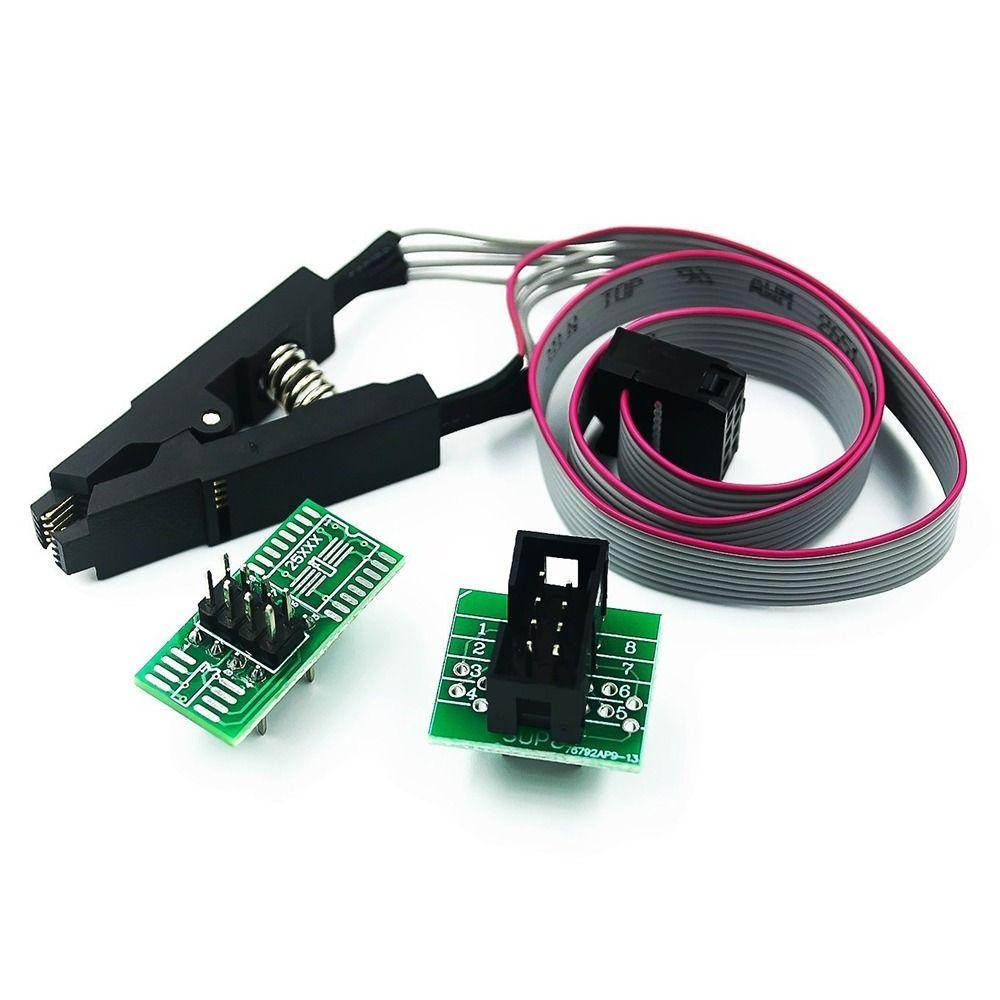
\includegraphics[width=0.4\textwidth]{images/device/programmer.jpeg}
    \caption{Programador \est{SOC8} amb pinça.}
    \label{fig:programmer}
\end{figure}

Per programar per \acro{isp} s'ha utilitzat una placa Arduino amb el codi
\est{ArduinoISP}, disponible a la mateixa aplicació \est{ArduinoIDE}
\cite{ArduinoIsp}. Un cop
l'Arduino tenia aquest codi, s'ha afegit una simple comanda d'\est{avrdude} 
al \est{Makefile}, permetent la programació senzilla del dispositiu.

\section{Distribució d'actualitzacions de \est{firmware}}

Quan incrustar el programa no és una tasca trivial, cal preguntar-se què
passaria si  es vol actualitzar la versió del \est{firmware} per afegir
funcionalitats o corregir errors. Queda clar que els consumidors no disposaran
de l'enginy de la figura \ref{fig:programmer} ni dels coneixements necessaris
per poder-lo utilitzar, per això s'ha de tenir present alguna forma per
poder canviar el codi del microcontrolador.

Una de les solucions més senzilles és tornar a posar el \est{Bootloader} a la
placa. D'aquesta forma, es podrà programar mitjançant la mateixa connexió
\acro{usb}, com s'ha fet durant l'etapa de desenvolupament. L'únic inconvenient
d'aquest sistema és que el dispositiu tardarà més a funcionar «amb normalitat»
a causa del temps que tarda a executar-se aquest codi inicial.

Una altra solució, tot i que no és aplicable per al \est{hardware} creat en aquest
projecte, és afegir un botó a la \acro{pcb} que, si es prem més de tres segons,
atura el programa principal del dispositiu i inicia un programa que
fa la mateixa tasca que el \est{Bootloader}. Aquest botó també podria aportar
altres beneficis com, per exemple, configurar més fàcilment el dispositiu.

Finalment, s'ha decidit no incorporar cap \est{Bootloader} en aquesta primera
tirada de dispositius, a causa a la no imminent comercialització. Tot i això,
s'ha pres nota de la importància d'aquest aspecte per tenir-lo present per a
futures versions de la placa de circuit imprès.
